\section{Obtained Results}
\label{results}

As described in the previous section, power consumption and computer time for each of the devices and algorithm tested, using different population size for each of the experiments, are reported in Table~\ref{T:r_obtained} and Figure~\ref{fig:powerenergy}.  

Different features can be analyzed:  (i) device behavior when considering energy consumed by the algorithm per unit of time; (ii) total energy required to find a solution and (iii) the way population size influences the energy needs when looking for a solution.

If we focus first on the energy required by lilgp to be run in every device, we notice that raspberry pi and handled devices are the least demanding ones, requiring 20 times less energy to run the same algorithm when compared with more standard computers:  Mac, Laptop and blade system.

Secondly, when considering the total energy required to reach the solution for the problem, the Tablet device running Android is the device that provide the \textit{cheapest} solution, according to energy consumed, while blade and laptops are the more \textit{expensive} ones in every case.  Yet, if we only focus on computing time, then, the opposite is the case, and Mac, Laptop and Blade would be the preferred ones.  But given that we are looking for energy efficient ways of finding solutions by means of EAs, then raspberry pi and tablet are preferred.

Finally, we can also analyse the influence of population sizes in both the time to reach solutions.  In the experimental stage, the runs with smaller population sizes typically reach 500 generations, given that they cannot find the solution with that small number of individuals.  So we will focus on the runs with larger population sizes.  Thus, the energy consumed to reach that solutions, we see that it's better to use the 500 individuals instead of 1000.  As already described by Koza, 500 is an optimal size for the problem, and adding more individuals don't benefit the search process, quite the opposite, adds a burden that implies larger computing time.  Nevertheless, what is of interest in this preliminary analysis, is the behavior of every device when this parameter is changed in this sequential version of the algorithm:  we have recorded a change in power consumption for the laptop, mac and blade system, while no change is found for raspberry and quite small changes for the tablet;  and this again benefits the latests.  


\begin{table}[!t]
\caption{Time (in seconds) for an EA run on each system depending on the population size. The numbers denote the mean and the standard error of the mean for the 30 runs performed.}
\label{T:r_obtained}
\begin{tabular}{lrcrcrcrcrc}
&&\multicolumn{9}{c}{population size}\\
\cline{3-11}
System 		&~~& 100	&~& 200	&~& 400	&~& 500	&~& 1000\\
\hline
Raspberry Pi	&& 7.77 $\pm$ 1.31	&& 19.91 $\pm$ 2.41	&& 46.22 $\pm$ 4.01	&& 61.10 $\pm$ 7.19	&& 116.80 $\pm$ 13.55	\\
Laptop	&& 1.73 $\pm$ 0.31	&& 4.43 $\pm$ 0.54	&& 10.60 $\pm$ 0.97	&& 13.89 $\pm$ 1.68	&& 27.13 $\pm$ 3.36	\\
iMac	&& 1.38 $\pm$ 0.28	&& 3.69 $\pm$ 0.48	&& 8.98 $\pm$ 0.84	&& 11.74 $\pm$ 1.44	&& 22.95 $\pm$ 2.85	\\
Tablet	&& 4.43 $\pm$ 0.75	&& 4.85 $\pm$ 0.78	&& 35.68 $\pm$ 4.15	&& 36.17 $\pm$ 4.17	&& 68.70 $\pm$ 7.89	\\
Blade	&& 2.59 $\pm$ 0.53	&& 6.88 $\pm$ 0.91	&& 16.78 $\pm$ 1.59	&& 22.28 $\pm$ 2.77	&& 43.53 $\pm$ 5.48	\\
\hline
\end{tabular}
\end{table}

\begin{figure}[!t]
\subfloat[]{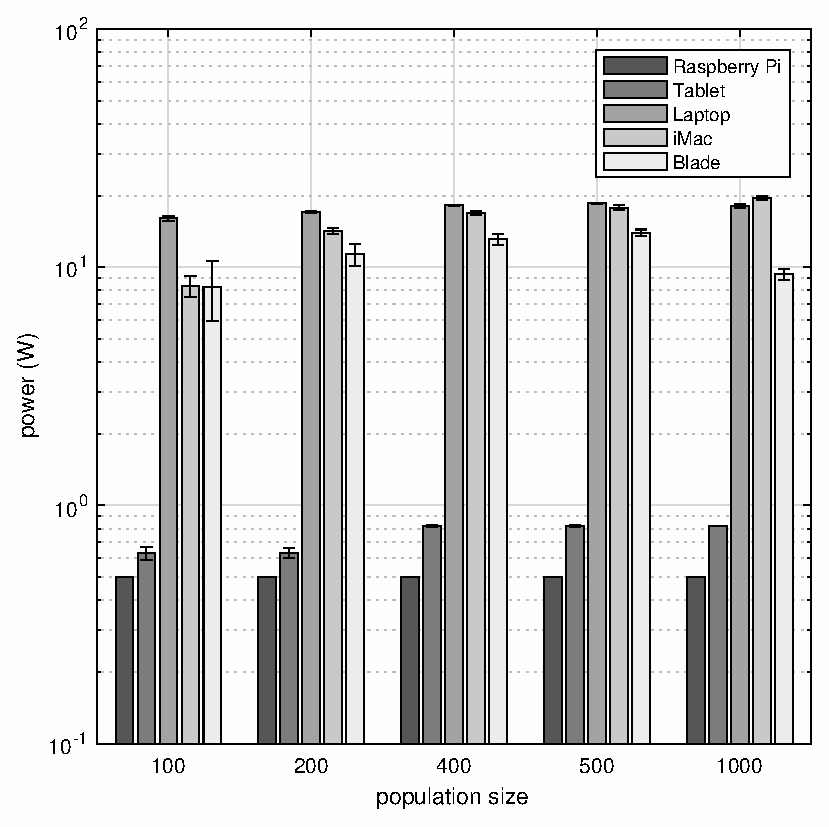
\includegraphics[width=.48\textwidth]{excess_power_log_2.eps}}~~
\subfloat[]{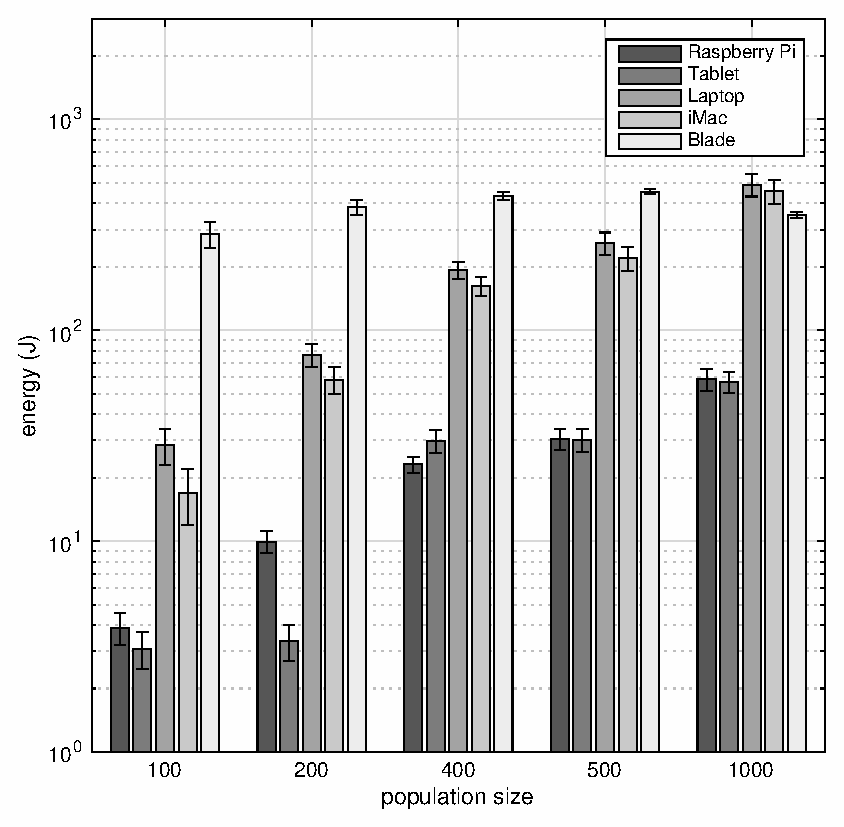
\includegraphics[width=.48\textwidth]{excess_energy_log_2.eps}}
\caption{(a) Instantaneous power delivered in each run. (b) Energy consumption per run. In both cases the bars (corresponding to raspberry pi, tablet, laptop, iMac and blade from left to right in each group) indicate mean values and the errorbars span the standard error of the mean. Notice the logarithmic scale in the Y axis.\label{fig:powerenergy}}
\end{figure}


\begin{figure}[!t]
\subfloat[]{\hspace{-1.1cm}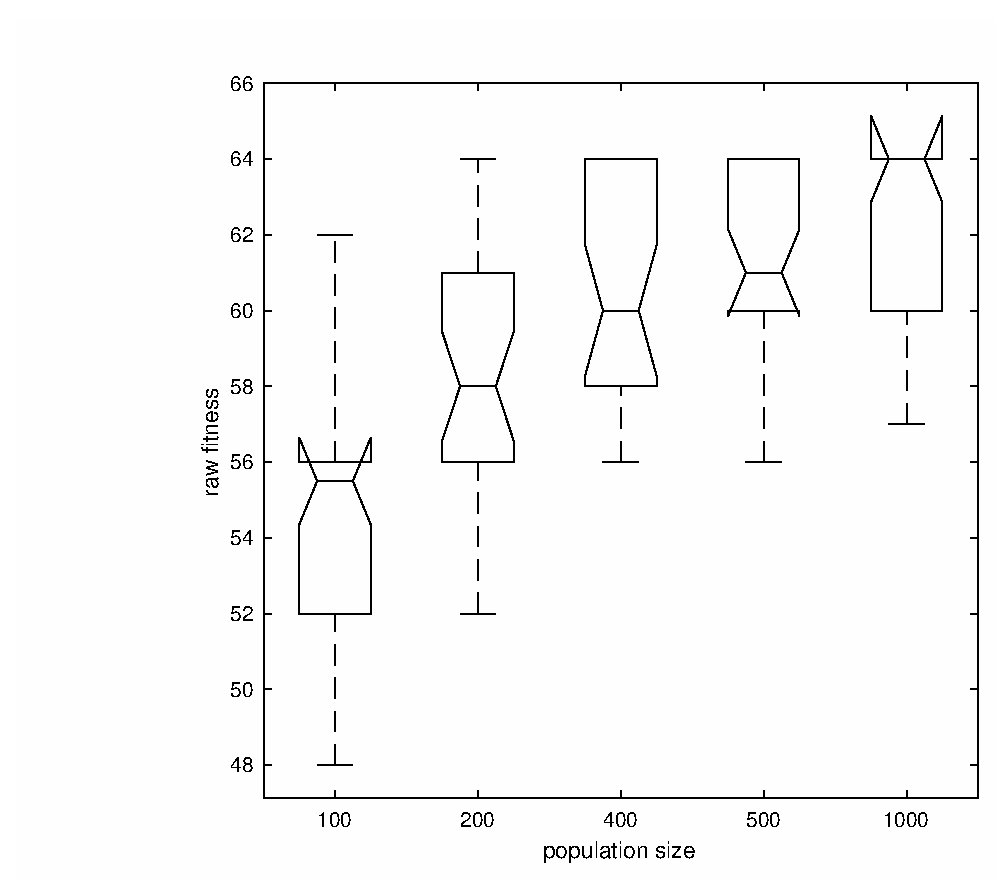
\includegraphics[width=.585\textwidth]{fitness.eps}}~~
\subfloat[]{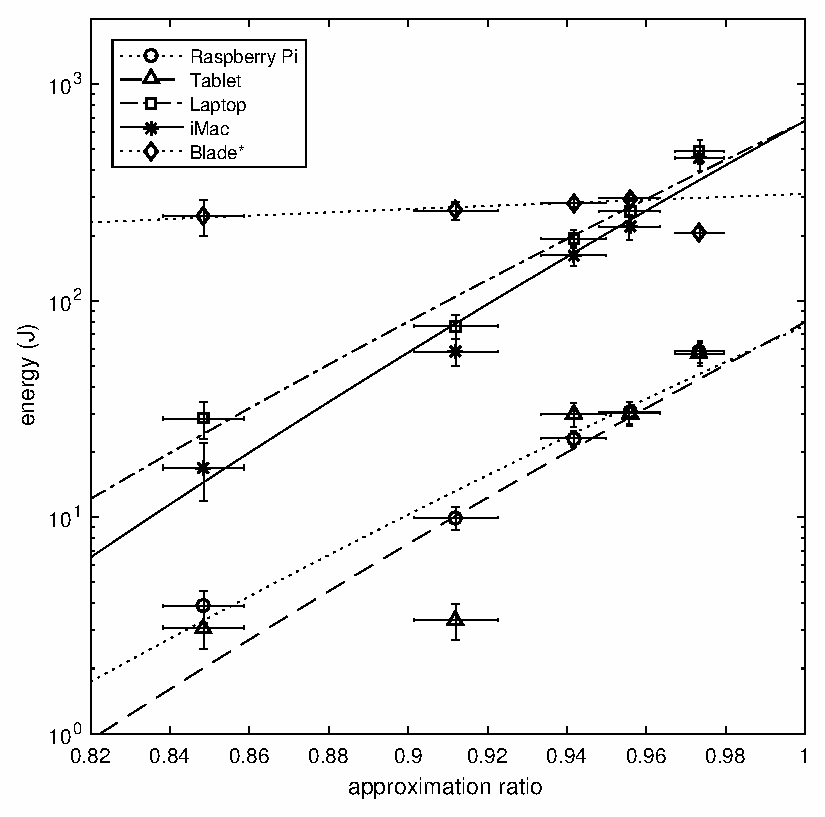
\includegraphics[width=.48\textwidth]{fitnessenergy.eps}}
\caption{(a) Distribution of fitness values attained for each population size (platform independent). 
(b) Tradeoff between fitness attained and energy consumption. The data points mark mean values and the error bars indicate the standard error of the mean. A fit to a power-law $E\propto f^k$ is also included (in the case of the Blade system, we have omitted the last point from the fit since it is clearly an outlier). 
\label{fig:fitnessenergy}}
\end{figure}

%We may notice first large differences in energy required to run the GP algorithm, when different hardware devices are employed.  Thus, raspberry pi and tablet devices are the ones requiring smaller ammounts of energy per unit of time (power).  Nevertheless, when we take into account not only power, but also total time to complete an experiment, and given that laptops and blade systems provide better computing capabilities, things could be different.  N


 %(~\ref{fig:consumo}). 

%\begin{figure}[ht]%
	%\centering
 	%\includegraphics[width=0.3\textwidth]{./Resultados/consumos.pdf}
 	%\caption{Consumo (w) del SoC en la implementación final del algoritmo.}
  %\label{fig:consumo} 
%\end{figure}



%\begin{figure}[ht]%
	%\centering
 	%\includegraphics[width=0.3\textwidth]{./Resultados/voltimetro.pdf}
 	%\caption{Voltímetro utilizado para la toma de medidas de potencia en los resultados experimentales.}
  %\label{fi:voltimetro} 
%\end{figure}


%Table~\ref{Table:result_todos} shows results obtained with a population size of 100, 200, 400, 500 and y 1000 individuals, respectively. 

%\begin{small}
%
%\begin{table}[!ht]
%\renewcommand{\arraystretch}{1.3}
%\centering
%\caption{Experimental results - GP - Multiplexer 6}
%\label{Table:result_todos}
%\begin{tabular}{ccccc} \hline
%Device & Power (W) & Time (sec.) & Energy (Joules) & (Kwh) \\ \hline
%\multicolumn{4}{c}{\textbf{Population size = 100}}\\ %\hline
%Raspberry Pi & 0.5 & 233.14 &116.57 & $3.24*10^{-5}$ \\
%Tablet & 0.63 & 132.75 & 83,3 & $2.31*10^{-5}$ \\
%Mac & 12.26 & 41.51 & 508,91 & $1.41*10^{-4}$ \\
%Laptop & 16.49 & 51.79 & 853.95 & $2.37*10^{-4}$ \\
%Blade & 13.8 & 77.84 & 1074.19 & $2.98*10^{-4}$ \\ \hline
%\multicolumn{4}{c}{\textbf{Population size = 200}}\\ %\hline
%Raspberry Pi & 0.5 & 597.29 & 298.64 & $8.30*{-5}$ \\
%Tablet & 0.63 & 145.63 & 92.9 & $2.56*10^{-5}$ \\
%Mac & 14.87 & 110.58 & 1644.32 & $3.77*10^{-4}$ \\
%Laptop	& 17.38 & 132.88 & 2309.41 & $6.42*10^{-4}$ \\
%Blade & 18.71 & 206.48 & 3863.24 & $1.07*10^{-3}$ \\ \hline
%\multicolumn{4}{c}{\textbf{Population size = 400}}\\ %\hline
% Raspberry Pi & 0.5 & 1386.52 & 693.26 & $1.93*10^{-4}$ \\
%Tablet & 0.82 & 1070.26 & 873.1 & $2.43*10^{-4}$\\
%Mac&17.49 & 269.38 & 4711.68 & $1.11*10^{-3}$\\
%Laptop & 18.25 & 317.98 & 5803.17 & $1.61*10^{-3}$\\
%Blade & 21.17 & 503.33 & 10655.5 & $2.96*10^{-3}$ \\ \hline
%\multicolumn{4}{c}{\textbf{Population size = 500}}\\ %\hline
%Raspberry Pi & 0.5 & 1833.07 & 916.53 & $2.55*10^{-4}$ \\
%Tablet & 0.82 & 1085.17 & 890.56 & $2.47*10^{-4}$ \\
%Mac & 18.75 & 352.31 & 6605.81 & $1.83*10^{-3}$ \\
%Laptop & 18.58 & 416.76 & 7743.73 & $2.15*10^{-3}$ \\
%Blade & 22.19 & 668.54 & 14834.90 & $4.12*10^{-3}$ \\ \hline
%\multicolumn{4}{c}{\textbf{Population size = 1000}}\\ %\hline
%Raspberry Pi & 0.5 & 3504.14 & 1752.07 & $4.87*10^{-4}$ \\
%Tablet & 0.82 & 2060.85 & 1686.49 & $4.68*10^{-4}$ \\
%Mac & 19.89 & 688.63 & 13696.85 & $3.80*10^{-3}$ \\
%Laptop & 19.01 & 813.78 & 15469.93 & $4.30*10^{-3}$ \\
%Blade &	17.1 & 1305.84 & 22329.86 & $6.20*10^{-3}$ \\ \hline
%
%\end{tabular}
%\end{table} 
%\end{small}


%Table~\ref{Table:result_ga} shows GA results when using population sizes: 50, 100, 500 y 1000.

%\vspace{-0.5cm}
%\begin{table}[!ht]
%\renewcommand{\arraystretch}{1.3}
%\centering
%%\tiny
%\caption{Experimental Results - GA}
%\label{Table:result_ga}
%\begin{tabular}{cccc} \hline
%Device & Power (W) & Time (seg.) & Energy (Kwh) \\ \hline
%\multicolumn{4}{c}{\textbf{Population size = 50}}\\ %\hline
% Raspberry Pi & 0,32 & 41,66 &  $0,370*10^{-5}$ \\
% Laptop & 12,76 & 5,1 & $1,81*10^{-5}$ \\
% Smartphone & 0,27 & 35,48 & $0,272*10^{-5}$ \\
% FPGA & 1,982 & 60,523 & $3,332*10^{-5}$\\  \hline
%\multicolumn{4}{c}{\textbf{Population size = 100}}\\ %\hline
% Raspberry Pi & 0,32 & 109,89 &  $0,977*10^{-5}$ \\
% Laptop & 15,76 & 12,11 & $5,3*10^{-5}$ \\
% Smartphone & 0,26 & 65,75 & $0,48*10^{-5}$ \\
% FPGA & 1,990 & 153,06 & $8,4608*10^{-5}$ \\ \hline
%\multicolumn{4}{c}{\textbf{Population size = 500}}\\ %\hline
% Raspberry Pi & 0,38 & 996,61 &  $10,520*10^{-5}$ \\
% Laptop & 18,6 & 87,16 & $45,034*10^{-5}$ \\
% Smartphone & 0,18 & 802,26 & $4,185*10^{-5}$ \\
% FPGA & 2,050 & 964,27& $54,909*10^{-5}$\\ \hline
%\multicolumn{4}{c}{\textbf{Population size = 1000}}\\ %\hline
% Raspberry Pi & 0,5 & 2572,8 &  $35,733*10^{-5}$ \\
% Laptop & 19,49 & 215,33 & $116,475*10^{-5}$ \\
% Smartphone & 0,22 & 2219,80 & $13,807*10^{-5}$ \\
% FPGA & 2,172 &2429,97 & $146,60*10^{-5}$\\ \hline
%\end{tabular}
%\end{table} 
%%\vspace{-0.5cm}


